\section[\thesection \  Hardware]{Hardware}\label{sec:hardware}

% Frame 4
\begin{frame}{Intel Neural Compute Stick 2}
    \begin{columns}[T]
        \column{0.6\textwidth}
        Beschleuniger für die Inferenz von Deep Learning Algorithmen
        \vspace{0.3cm}
        \begin{itemize}
            \item geeignet für \textbf{Edge Anwendungen} wie:
            \begin{itemize}
                \item Überwachungskameras, Drohnen, \dots
            \end{itemize}
            \end{itemize}
            \begin{itemize}
                
            
            \item Prozessor: \textbf{Intel Movidius Myriad X VPU}
            \begin{itemize}
                \item effizient bei NN-spezifischen Rechenopereationen
            \end{itemize}
            
        \end{itemize}
        \column{0.4\textwidth}
        \vspace{1cm}
        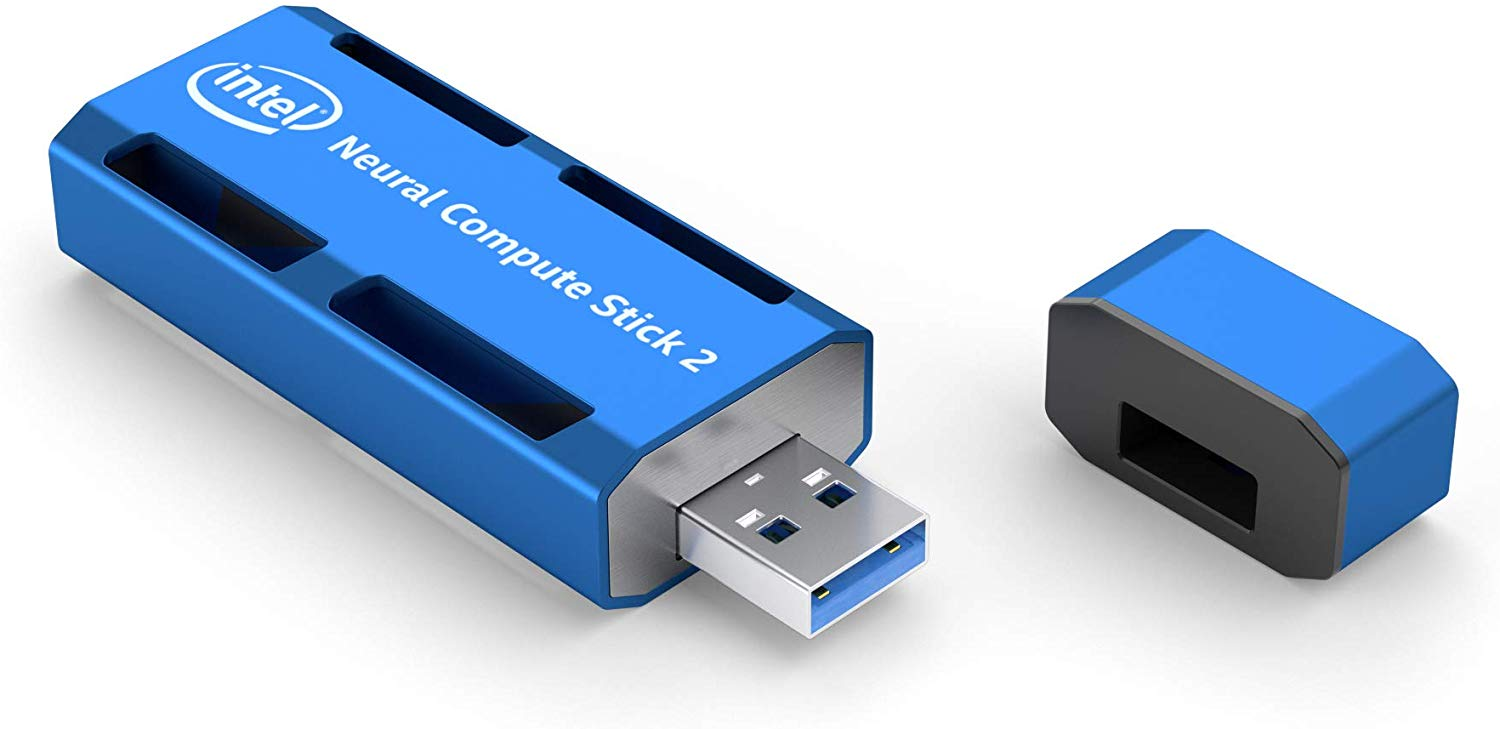
\includegraphics[width=0.8\textwidth]{Bilder/ncs2.jpg}
    \end{columns}
    \vspace{0.3cm}

    \visible<2->{

    \begin{columns}[T]
        \column{0.4\textwidth}

        \begin{block}{OpenVINO Toolkit}
    
            Inferenz auf Intel-Hardware
            \begin{itemize}
                \item Eigenes Dateiformat für Deep Learning Model
                \item Unterstütze Frameworks:
                \begin{itemize}
                    \item  Tensorflow, Caffe
                \end{itemize}
            \end{itemize}
        \end{block}
            \column{0.6\textwidth}
            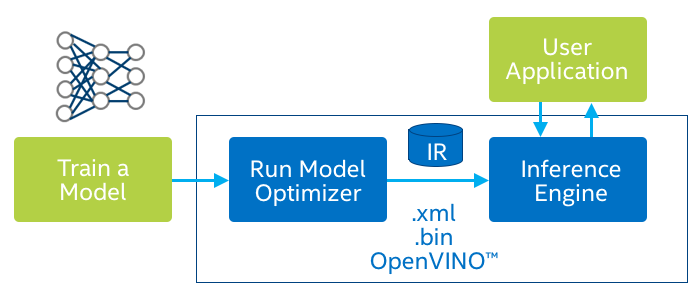
\includegraphics[width=\textwidth]{Bilder/open_vino_workflow_steps.png}
        \end{columns}

    }
        
\end{frame}